% Derived from nn_graphics (MIT) for residual block styling.
\documentclass[border=6pt]{standalone}
\usepackage{tikz}
\usetikzlibrary{arrows,positioning,calc,chains,scopes}

\definecolor{layerblue}{RGB}{200,220,255}
\definecolor{layergreen}{RGB}{210,240,210}
\definecolor{layerorange}{RGB}{255,235,200}
\definecolor{layergray}{RGB}{230,230,230}

\tikzstyle{signal}=[arrows={-latex},draw=black,line width=1.2pt,rounded corners=3pt]
\tikzstyle{layer}=[draw=black,fill=layergray,minimum width=90pt,minimum height=16pt,font=\footnotesize]
\tikzstyle{conv}=[layer,fill=layergreen]
\tikzstyle{bn}=[layer,fill=layerblue]
\tikzstyle{activation}=[layer,fill=layerorange]
\tikzstyle{point}=[circle,draw=black,fill=layergray,minimum size=16pt,font=\footnotesize]
\tikzstyle{branch}=[coordinate]

\begin{document}
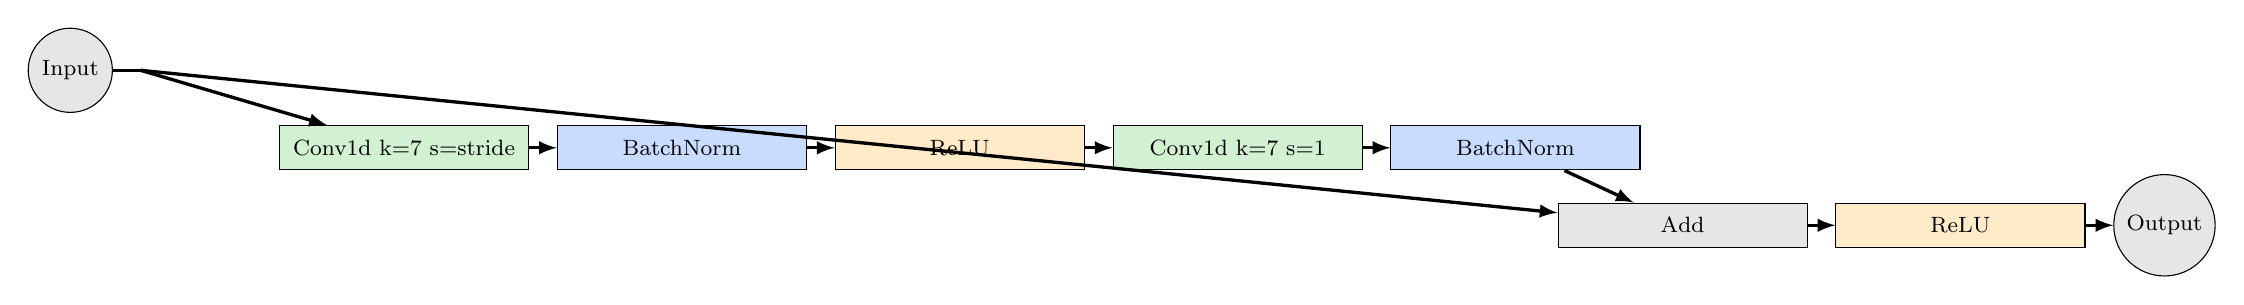
\begin{tikzpicture}[
    start chain=going right,
    node distance=10pt,
    layer/.append style={on chain, join=by {signal}},
    point/.append style={on chain, join=by {signal}},
    branch/.append style={on chain, join=by {signal, -}},
]
    \def\branchy{28pt}

    \node[point] {Input};
    \node[branch] (skip) {};
    \node[conv, xshift=40pt, yshift=-\branchy] {Conv1d k=7 s=stride};
    \node[bn] {BatchNorm};
    \node[activation] {ReLU};
    \node[conv] {Conv1d k=7 s=1};
    \node[bn] {BatchNorm};
    \node[layer, xshift=-40pt, yshift=-\branchy] (add) {Add};
    \node[activation] {ReLU};
    \node[point] {Output};

    \draw[signal] (skip) -- (add);
\end{tikzpicture}
\end{document}
